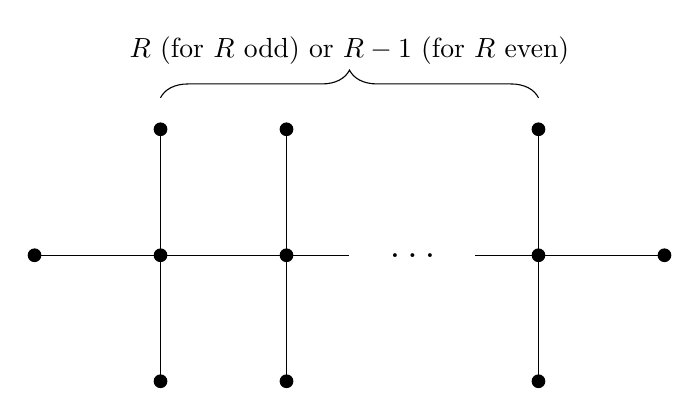
\begin{tikzpicture}[scale=1.6]
\foreach \x in {0,1,2,4,5}
{
  \draw[fill=black,draw=black] (\x cm, 0) circle (.5mm) ;
}
\draw (0,0)--(1,0)--(2,0)--(2.5,0);
\draw (3.5,0)--(4,0)--(5,0);
\node at (3,0) {\Large{$\ldots$}};
\foreach \x in {1,2,4}
{
  \draw[fill=black,draw=black] (\x cm, 1) circle (.5mm) ;
	\draw[fill=black,draw=black] (\x cm, -1) circle (.5mm) ;
	\draw (\x,1)--(\x,0)--(\x,-1);
}
\draw [decorate,decoration={brace,amplitude=10pt}] (1,1.25) -- (4,1.25) node [black,midway,yshift=17]  {$R$ (for $R$ odd) or $R-1$ (for $R$ even)};
\end{tikzpicture}